

\documentclass[a4paper]{scrartcl}

% Mathematik-Pakete
\usepackage{amsmath}
\usepackage{amssymb}
\usepackage{amstext}
\usepackage{amsfonts}
\usepackage{mathrsfs}
\usepackage{paralist}
\usepackage[pdftex]{graphicx}
\usepackage{fancyhdr}
\usepackage{color}



%\usepackage[ansinew]{inputenc}
%\usepackage[T1]{fontenc}

\usepackage[utf8]{inputenc}
%\usepackage[latin1]{inputenc}  
%\usepackage[T1]{fontenc}
%\usepackage{lmodern}          
\usepackage[a4paper]{geometry}
\geometry{verbose,tmargin=1.5cm,lmargin=2cm,rmargin=2cm,bmargin=2cm,nohead}
\usepackage[ngerman]{babel}
\setlength{\parindent}{0cm}


\begin{document}
\pagestyle{fancy}
\setlength{\footskip}{10mm}
\fancyhf{}
\renewcommand{\headrulewidth}{0pt}
\renewcommand{\footrulewidth}{0.5pt}

%\twocolumn[
 \centerline{\LARGE \bf \textsf{MSE CFD}} 
 \smallskip
\centerline{\Large \bf \textsf {Zusammenfassung}}
\medskip
  \centerline{\bf \textsf{dstrebel, s1bischo, sboller }}

 \smallskip \noindent\rule{\textwidth}{0.5pt}
\smallskip%]

\section{Conservation laws of fluid motion and boundary conditions}
\subsection{Conservation Euqations}
Explain the physical meaning of the different terms in the conservation
equations (link between mathematical “operations” and physical behaviour)

Präsentation Folie 7

Impulsgleichung


Energiebilanz

\begin{table}[h]
\begin{center}
\begin{tabular}{|l|l|}
\hline Continuity & $\frac{\partial(\rho)}{\partial t}+\operatorname{div}(\rho
\vec u)=0$
\\
\hline x-Momentum & $\frac{\partial(\rho u)}{\partial
t}+\operatorname{div}(\rho u \vec u) = - \frac{\partial p}{\partial
x}+\operatorname{div}(\mu \operatorname{grad} u)+S_{Mx}$ \\
\hline y-Momentum & $\frac{\partial(\rho v)}{\partial
t}+\operatorname{div}(\rho v \vec u) = - \frac{\partial p}{\partial
y}+\operatorname{div}(\mu \operatorname{grad} v)+S_{My}$ \\
\hline z-Momentum & $\frac{\partial(\rho w)}{\partial
t}+\operatorname{div}(\rho w \vec u) = - \frac{\partial p}{\partial
z}+\operatorname{div}(\mu \operatorname{grad} w)+S_{Mz}$ \\
\hline Energy & $\frac{\partial(\rho i)}{\partial
t}+\operatorname{div}(\rho i \vec u) = -p \operatorname{div} \vec u +
\operatorname{div}(k \operatorname{grad} T) + \Phi + S_i$ \\
\hline Equations of State & $p=p(\rho, T)$ und $i=i(\rho, T)$ \\
\hline
\end{tabular}
\caption{Governing Equation of the flow of a compressible Newtonian fluid}
\end{center}
\end{table}


\subsection{Explain the physical meaning of the different terms in a general
transport equation}

\begin{align}
\frac{\partial(\rho \phi)}{\partial t} + \operatorname{div}(\rho\phi\vec
u)=\operatorname{div}(\Gamma \operatorname{grad} \phi) + S_\phi
\end{align}

\begin{table}[h]
\begin{center}
\begin{tabular}{|p{3cm}|p{3cm}|p{3cm}|p{3cm}|}
\hline Rate of increase of $\phi$ of fluid element +& Net rate of flow of $\phi$
out of fluid element =& Rate of increase of $\phi$ due to diffusion +& Rate of
increase of $\phi$ due to sources \\
\hline Zeitliche Änderung von $\phi$  +& Konvektiver Transport: Fluss von $\phi$
mit der Strömung =& Diffusiver Transport: Transport von $\phi$ aufgrund von
Konzentrationsunterschieden (grad). Diffusionskonstante $\Gamma$ bestimmt Menge
+& Quellterm innerhalb des Fluidelements \\
\hline
\end{tabular}
\caption{Meaning of general transport equation}
\end{center}
\end{table}

Derive continuity and momentum equations from basic physical idea (mass conservation, Newton second law) and general transport equation with appropriate variable substitutions
Präsentation Folie 5

Kontinuitätsgleichung bedeutet Qellenfrei, Erhaltend





\section{Turbulence and its modelling}

\subsection{Properties of turbulence}
Explain the properties of turbulence and their influence on the flow
field. Which changes can be observed compared to laminar flow?

\textbf{Turbulence is irregular, disorderly, non-stationary, three-dimensional,
highly non-linear, irreversible phenomenon}

\begin{itemize} 
\item Nichtlinear
\item Zufälligkeit (nicht Reproduzierbar)
\item 3D, auch wenn Mittelwert in 1D und 2D variert
\item hohe Wirbelstärke
\item Energie wird dissipiert (wird immer kleiner)
\item Intermittency: Turbulenz kann nur in Teilen der Strömung vorhanden sein.
$\Rightarrow$ Eine Strömung kann nicht nur aus turbulenten Anteilen bestehen.
\item Hohe Diffusivität von Impuls und Energie (Gute Verteilung)
\item Turbulenz ist lokaler Umgebung abhängig (z.B. Absatz)
\end{itemize}
\subsection{RANS and LES Modelling}
Explain the main approximations using RANS
and LES modelling, including assumptions (what is computed and how, what is modelled and how)
\subsubsection{RANS}
\textbf{Reynolds-averaged Navier–Stokes (RANS)}

RANS besteht aus einem Mittelwert der Strömungskennwerte und einem stochastisch
fluktuierenden Anteil. Vor der numerischen Berechnung der Lösung liegen die
Navier-Stokes Gleichungen als zeitgemittelt vor. Nichtlineare Extraterme liegen
in den RANS aufgrund der Interaktionen der verschiedenen turbulenten Fluktuationen vor.
Diese werden normalerweise mit klassischen Turbulenzmodellen wie dem
$k-\epsilon$- oder dem Reynoldsstress-Modell modelliert.
\\
\textit{Vorteile:} erträgliche Rechenleistung bei brauchbaren Resultaten,
deshalb die meistverwendete Methode. \\
\vspace{0.5cm}
\textbf{Large Eddy Simulation}
Nur grosse Turbulenzelemente werden exakt aufgelöst. Kleinere Turbulenzelemente
werden über Filterfunktionen herausgefiltert. Diese nicht direkt berechneten
Elemente werden über sogenannte Subgrid-Scale Models approximiert. \\
\vspace{0.5cm}
\textit{Vorteile:} Bessere Resultate insbesondere bei komplexen Geometrien. \\
\textit{Nachteile:} Grösserer Speicher- und Rechenzeitbedarf



\subsection{Wallfunctions} 
Im Engineeringbereich interessieren die Details der Near-Wall Region im
Normalfall nicht. Von Interesse ist hingegen der Strömungswiderstand in der Nähe
der Wände. Wallfunktionen korrigieren die \colorbox{red}{bla bla bla}s

What are wall functions, idea behind them, advantages
and disadvantages tabelle funktion


wandfunktion bei hohen reynoldzahl vereinfacht komplexität
dimensionlose Kennzahl der Abstand der ersten Zelle am Rand, siehe Bild Silvio



\section{The finite volume method for the diffusion problem}


\subsection{FV Discretisation for a one-dimensional heat conduction Problem}
Derive a finite-volume discretization for a one-dimensional heat conduction
problem. 

\begin{figure}[h]
\begin{center}
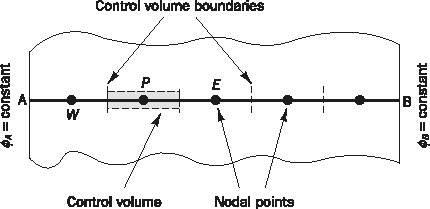
\includegraphics[scale=1]{images/41.pdf}
\caption{One-Dimenstional Heat Conduction}
\label{fig:Kreisel}
\end{center}
\end{figure}


\begin{itemize}
\item Derive a finite-volume discretization for a one-dimensional heat conduction problem. 

mit Unterlagen... Folie 14

\item Demonstrate, using Taylor series expansion, that the central differencing scheme has second order accuracy.

Folie 11, siehe auch Multiphysik


\end{itemize}




\section{5 The finite volume method for convection-diffusion problems}
\begin{itemize}
\item Explain why the CDS (central differencing scheme) does not work for large velocities.
Pe - Klee Zahl verhänihs zeischen Konvektion und Diffusion
Internet

\item Define the Peclet number
Pe - Klee Zahl verhänihs zeischen Konvektion und Diffusion

\item Explain why the upwind discretization (UD) works better. Explain the disadvantages of upwind discretization.
Richtung im Wind, 
disadvatianges:
- es leidet von falscher numerischer
- ist nur 1 ordungng und eshalb eher ungenau
advatianges
- grosse Zeitschritte
- schlechteres netz
- 



\item Explain the terms: conservativeness, boundedness, transportiveness
nachlesen...



\item Explain how the hybrid differencing scheme works.
idea: kombination von upwind und central, 1 Ordnung....
upwind: hoche PeKlee Zahen (hohe konvektion und wenig diffusion)
centrel diffenzing: kleine PeKlee Zahlen (weil mehr diffusion)

\item Explain the QUICK scheme. Advantages and disadvantages.
optimierung von upwind, schaut noch weiter in Zukunft und gewichtet die Zukunft
sehr negativ ist es überschwingt, dies ist total unphysikalisch
positiv näher an der exakten lösung




\item Describe the idea behind TVD schemes.
TVD steht für Total Vaariation Diminishing,
Ideeist die Hügel zu reduzieren
Folie 19



\end{itemize}



\section{6 Solution algorithms for pressure velocity coupling in steady flows}
\begin{itemize} 

\item Difference between incompressible (pressure-based) and compressible (density based) approach/codes => which equations are available for which variable
incompressibel, dichteänderung gleich 0 und p ist konstant
compressible, dichteänderung ...
folen 7


\item Differences between momentum equations and general scalar transport equations => new aspects to be tackled
??? zu folie 11

\item Explain the SIMPLE procedure for pressure-velocity coupling
siehe folie 14

\item Explain the role of relaxation factor. 
Flussdiagramm siehe Folie 14


\item Why are they used?
folie 20


\end{itemize}



\section{7 Solution of discretized equations}
\begin{itemize}
\item Explain why iterative methods are necessary to solve sparse linear systems.
schneller gelöst, numerisch weniger aufwindig
Iterative löser ...
sparse linear system sind einfach pararellisierbar


\item Describe the Jacobi and Gauss-Seidel iterative methods
Jacobi iterative method: 
möglichst nahe an einheitsmatix kommen
eigenwert muss keiner 1 sein, wird dafür langsamer 

Gauss- Seidel method: 
nicht paararellisierbar, konvergit schneller

\item Describe the idea behind the multi-grid method
Anfangsbedingungne 
Stufenweises lösen auf verschiednen netzgrüssen
foleie 19 (Ansys arbeitet so)
feien lösen
grobes netzt lösen
dann wieder feiner...

\end{itemize}



\section{8 The finite volume method for unsteady flows}
\begin{itemize}
\item Describe the three common schemes for time discretization:
\begin{itemize}
\item Explicit (forward Euler)
...

\item Cranck-Nicholson
...

\item Implicit (backward Euler)
...

\end{itemize}
\item What are the advantages and disadvantages of the different schemes?


\item How does the SIMPLE scheme have to be modified for a transient simulation?



\end{itemize}





\section{9 Implementation of boundary conditions}
\begin{itemize}

\item Name 5 important boundary conditions
Dirichlet boundary conditions
Neumann boundary conditions
Robin bandary  condition


inelt
outlet
wall



\item Why cannot symmetry planes (and symmetry boundary conditions always be used in 
CFD)?
\item Why should outlets be placed far away from the interesting flow region?
weil am anfang am rand falsche randbedingungen sind, siehe bild silvio, slide 38


\end{itemize}


\section{10 Errors and uncertainty in CFD modelling}

\begin{itemize}
\item Describe three potential numerical errors in CFD

\begin{itemize}
\item Disketierungsfehler (netzt ist nicht perfekt ist wenn abgeschitten wir
\item Rundungsfehler (flot...)
\item Iterative Konvergenzfehler, Residien???
\end{itemize}
siehe buch 289

\item Describe two typical physical uncertainties in CFD (uncertainties = Unsicherheiten)
limitierte genauigkeit
submodell ist nicht vallierdt
siehe Buch 291

\item What do the terms verification and validation mean.
verification, mathematisch teil, ...
validation, ingenieur, überprüfen von beschreibung der wirklichkeit entspricht


\end{itemize}



Hier eine Mustergleichung... :-) von PartDiff :-)
\[
\frac{\partial^3 u}{\partial x^3}-\frac{\partial u}{\partial y}=0
\]




\end{document}




